% figures/app-beijing.tex -- Figure S1 do supp_5.tex, Secao S10 (E5h, 2026-10-06;
% D21, D57). A figura e a beijing.heat.pdf do compendio (R/application_report.R).
% Duas escolhas de apresentacao da E5h, a confirmar na E5b: (i) a linha do nivel
% (o intercepto a vento zero, 0 C e 1000 hPa) nao e desenhada (D67(f)), o que pede
% tirar a linha `one` da figura no compendio; (ii) a borda da umidade se decide
% depois da rodada (D67(e)). As marcas da temporada sao as nominais (D66).
% E5k (2026-10-08): a caixa virou a figura, copia de results/figures/beijing.heat.pdf
% (refeita depois do piloto: o rug, D75(e), e a umidade cortada a ~15% e ~95%,
% `trim: rh: [6, 4]` do application.yaml, D67(e)). A figura do compendio ainda tem a
% linha do nivel; ate o compendio ter a opcao sem ela (handoff-E5k.md), o recorte
% abaixo a tira sem mexer no PDF: a faixa da legenda (do topo ate 22 bp) e as tres
% linhas de baixo (de 218 bp ate o fim), na pagina de 518 x 806 bp do PDF; as duas
% medidas caem em faixas brancas (pdftoppm a 72 dpi). Quando o compendio tirar a
% linha, volta a um \includegraphics so. A legenda segue a da Figure 2 (D68(g), E5j):
% os tipos de linha saem (a legenda do PDF os nomeia), "band" no lugar de "grey", os
% cortes ditos; o achado fica no texto da S10, como o da Figure 2 no 6.3 (a legenda com
% ele passava 98 pt da pagina). \color{colR1} dentro do float (D75(d)).
\begin{figure}[tp]
\color{colR1}
\centering
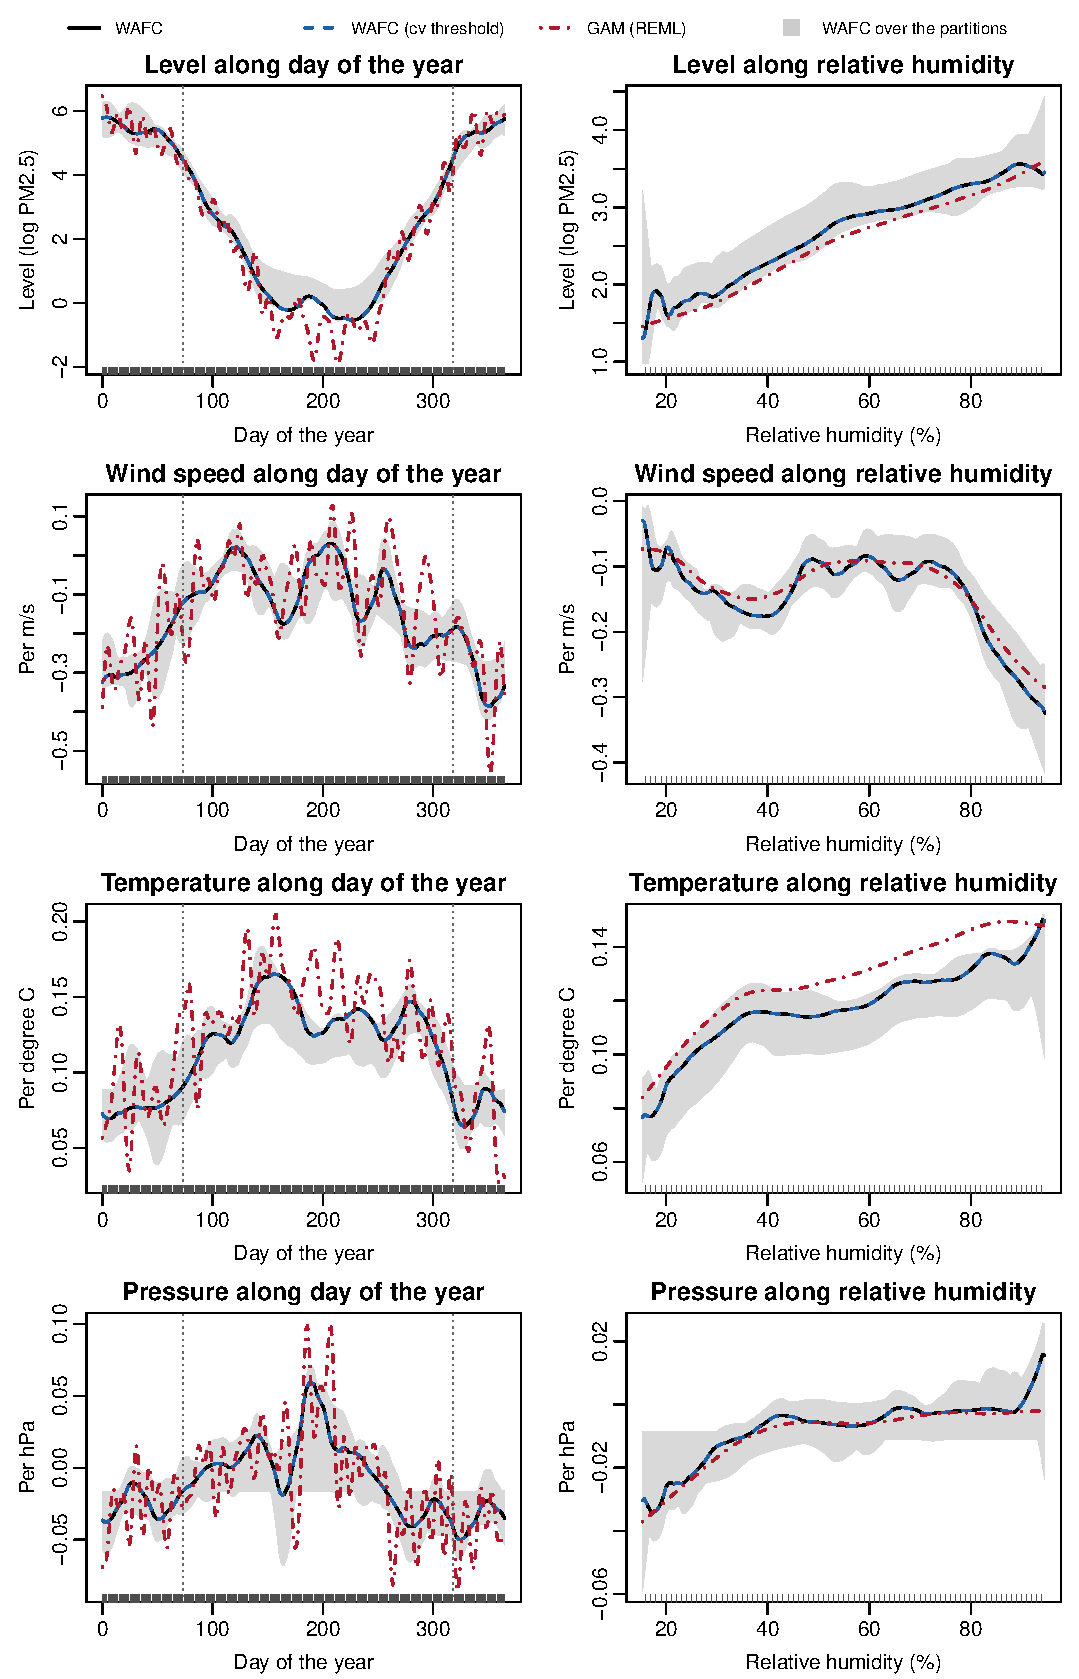
\includegraphics[width=0.72\textwidth,trim=0 784 0 0,clip]{figures/beijing.heat.pdf}\\
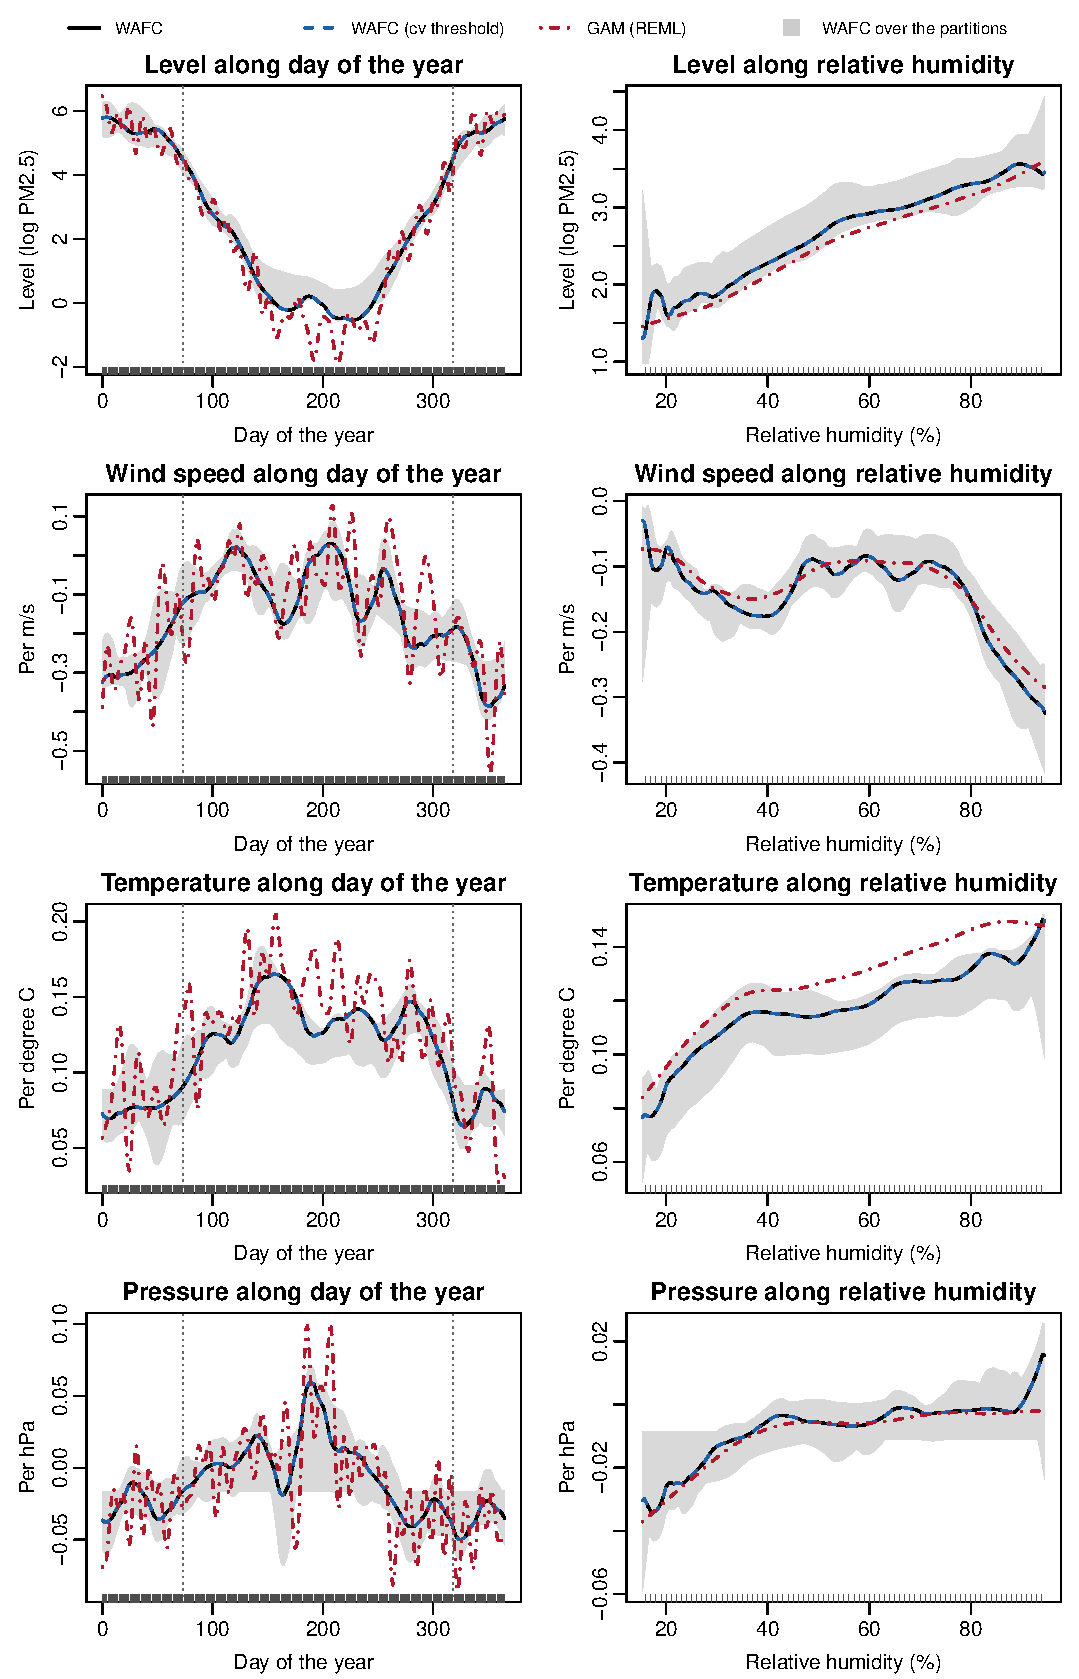
\includegraphics[width=0.72\textwidth,trim=0 0 0 218,clip]{figures/beijing.heat.pdf}
\caption{Beijing, Dongsi, hourly, March 2013 to February 2017: the
coefficients of the wind speed (top, per m/s), the temperature (middle, per
$^{\circ}$C) and the pressure (bottom, per hPa) for the logarithm of PM2.5,
along the day of the year (left) and the relative humidity (right), with the
component of the other modulator at its sample mean; the band is the range
of the WAFC over 20 fits on 70\% of the weeks, and the vertical lines mark
the nominal heating season, 15 November to 15 March. Not shown: the level,
which moves along the year with the coefficient of the temperature, and the
relative humidity below about 15\% and above about 95\%, where the
periodized basis joins the two ends of its range; ticks on the axes mark the
observed values.}
\label{fig:beijing}
\end{figure}
